\chapter{Global Event Reconstruction}

% https://doi.org/10.1088/1748-0221/12/10/P10003

In the previous chapter, we discussed the interactions of particles with the individual subdetectors and how these generate electrical signals.
Now, we shall discuss the reverse process, namely reconstructing the individual particles or physics objects from the electrical signals recorded by the subdetectors.

Traditionally, each class of physics object ia reconstructed using information from a single subdetector: muons from the muon chambers, isolated photons and electrons from the ECAL, jets and missing transverse energy from the HCAL, and secondary vertices from $\tau$ lepton and $b$ hadron decays from the tracker.
However, as depicted in Figure~\ref{fig:cms_slice}, each type of particle interacts with multiple different subdetectors and this information is lost unless the information from all the subdetectors is combined into a single global event description.

The particle flow (PF) algorithm leverages the fine angular granularity of the calorimeters and the excellent momentum resolution of the inner tracker and muon chambers to greatly improve the reconstruction of physics objects and include soft particles that would otherwise be ignored.
This is especially advantageous for jet energy measurements as roughly 62\% of the jet energy is carried by charged hadrons, approximately 27\% by photons, around 10\% by neutral hadrons, and about 1.5\% by neutrinos.

\begin{figure}[htbp]
  \begin{center}
    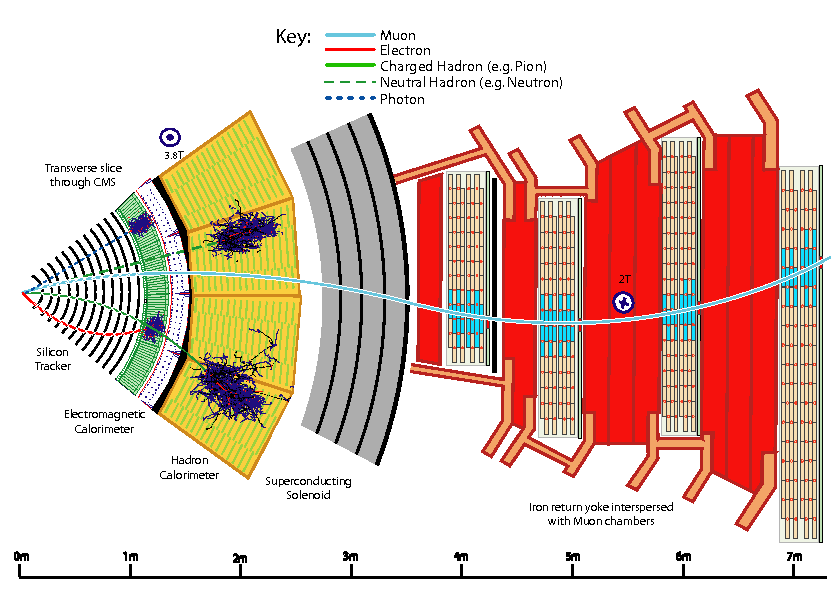
\includegraphics[width=0.875\textwidth]{Reconstruction/Figures/cms_slice.png}
    \caption{
      A sketch of a transverse slice of the CMS detector showing particle interactions from the interaction point to the muon detector.
      % Charge particles tracks are shown with solid lines while the paths of neutral particles are shown with dotted lines. 
      % The muon and charged pion are positively charged and the electron is negatively charged.
      % Neutrinos do not interact with the detector at an appreciably rate.
      Reprinted from Reference~\cite{}. % https://iopscience.iop.org/article/10.1088/1748-0221/12/10/P10003/meta
    }
    \label{fig:cms_slice}
  \end{center}
\end{figure}

The distinguishing feature of the PF algorithm is to combine multiple detector signals together into a single PF candidate.
The input detector signals are the tracks, vertices, calorimeter clusters, and muon segments described in Section~\ref{sec:pf_elements}.
Based on their proximity in the $\eta$-$\phi$, these PF elements are combined into muons, electrons, photons, and hadrons.
Muon segments are combined with inner tracks to produce muons, inner tracks are combined with calorimeter clusters to produce electrons and charged hadrons, and calorimeter clusters are correlated to produce photons and neutral hadrons.

The PF algorithm reconstructs particles in regions of the detectors called blocks following the steps described in Section~\ref{sec:pf_cands}.
After each step any PF elements associated to a PF candidate are removed from the block.
For example, clusters associated with photons will not be used when reconstructing neutral hadrons.
After all PF candidates are identified, they can be combined into event-wide variables such as jets and the missing transverse energy as described in Sections~\ref{sec:pf_jets} and~\ref{sec:pf_met}, respectively. 

\section{Particle Flow Elements}
\label{sec:pf_elements}

\subsection{Tracks}
\label{sec:pf_tracks}

% doi:10.1088/1748-0221/9/10/P10009

The Combinatorial Track Finder software is used to reconstruct tracks in an iterative inside-out process.
Initial interations search for tracks that are easy to find, e.g. those with high \pt, and hits associated with these tracks are removed for later iterations, reducing the combinatorial complexity and simplifying the search for more difficult tracks, e.g. greatly displaced ones.

The first step is to form seeds based on pixel hits, double strip hits containing 3D information, and an estimate of the beam spot.
Earlier iterations require three pixel hits while later iterations gradually loosen the requirements. %  to reconstruct displaced tracks.
The final iterations specifically target increased muon tracking efficiency by including information from the muon chambers.

Next, a Kalman filter is used to find additional hits consistant with the evolution of the track seeds through the rest of the tracker, accounting for the magnetic field, energy loss due to ionization, and multiple scattering.
The five parameters used for the helical trajectory evolution are the curvature $\rho$, the azimuthal angle $\phi_0$, the transverse impact parameter $d_0$ , the longitudinal impact parameter $z_0$ , and $\lambda = \cot \theta$, where $\theta$ is the polar angle.

After propagating the track through all layers of the detector and finding all associated hits, a Kalman fitter and smoother is used to refit the overall trajectory while a fourth-order Runge-Kutta method is used to extrapolate the trajectory between successive hits.
To reduce the fraction of fake tracks, various quality requirements concerning the number of missing hits, the reduced $\chi^2$ of the fit, and compatibility with a primary vertex are applied before proceeding to the next iteration.

% https://doi.org/10.1088/1748-0221/12/10/P10003

Track reconstruction for electrons is more complicated as the Kalman filter is not a good description because of the high rate of non-Gaussian energy loss due to brehmsstrahlung these tracks experience within the tracker.
To improve the electron reconstruction efficiency, the electron seed collection is filled both by looking outside-in for ECAL superclusters (see Section~\ref{sec:pf_sc}) consistant with track seeds and inside-out track seeds consistent with superclusters.
A Gaussian Sum Filter (GSF) defined to approximate the Bethe-Heitler energy-loss distribution is used to fit the trajectory of electron tracks. 

\subsection{Primary Vertexing}
\label{sec:pf_pv}

% doi:10.1088/1748-0221/9/10/P10009

A deterministic annealing (DA) algorithm is used to associate tracks to primary vertices.
Tracks must pass additional requirements on the transverse impact parameter $d_0$, the number of strip and pixel hits, and the reduced $\chi$ of the trajectory fit to be considered when finding primary vertices.
The most probable vertex positions at an artifical temperature $T$ are determined by the minimization of the ``free energy''
\begin{equation}
  F = -T \sum_i^{N_T} \ln \sum_j^{N_V} p_{ij} \rho_j \exp \left[ - \frac{1}{T} \left(\frac{z_i^T - z_j^V}{\sigma^z_i}\right)^2 \right]
\end{equation}
where the $z_j^V$ are the vertex positions with weights $\rho_j$, the $z_i^T$ and $\sigma_i^z$  are the longitudinal impact parameters and the corresponding uncertainties of the tracks, and the $p_{ij}$ are the probabilities of assigning the track $i$ of $N_T$ to the vertex $j$ of $N_V$.

The DA algorithm starts with a single vertex at a very high temperature that is gradually decreased.
The free energy $F$ is minimized with respects to $z_j^K$ at each new temperature and a vertex is split in two whenever $T$ falls below its criticial temperature
\begin{equation}
  T_C^j = 2 \sum_i \frac{p_i p_{ij}}{\left(\sigma_i^z\right)^2} \left(\frac{z_i^T - z_j^V}{\sigma^z_i}\right)^2 \Bigg/ \sum_i \frac{p_i p_{ij}}{\left(\sigma_i^z\right)^2}.
\end{equation}
The annealing procedure with vertex splitting continues down to $T = 4$ and the final assignment of tracks to vertices is performed at $T = 1$ without any further splitting. 
The vertex designated as \textit{the} primary vertex (PV) of the hard scattering is the one which maximizes
\begin{equation}
  S_T = \sum_i  (\pt^i)^2 + (\ptmiss)^2,
  \end{equation}
where $\pt^i$ is the transverse momentum of a track assigned to the vertex and \ptmiss\ is the magnitude of the momentum imbalance in the transverse plane for the vertex. 

\subsection{Secondary Vertexing}
\label{sec:pf_csv}

% https://arxiv.org/pdf/1712.07158.pdf

Long-lived particles such as $b$ hadrons and $\tau$ leptons often produce charged particles in their decays.
These charged particles are traced to a secondary vertex at the location of the decay, which is identified by the inclusive vertex fitter (IVF) algorithm.

The IVF procedure begins by selecting seed tracks with a 2D impact parameter significance $\sigma_{d_0} \ge 1.2$ and a 3D impact parameter $\sqrt{d_0^2 + z_0^2} \ge  50\mum$.
Tracks are assigned to a secondary vertex based on their opening angle with the seed track and distance at closest approach, with the additional stipulation that this distance be smaller for the secondary vertex than for the primary vertex.

To determine the precise position of the secondary vertices, the associated tracks are fitted with the adaptive vertex fitter and any vertices with a flight distance significance less than a certain threshold are discarded.
At this point, a track is unassociated from a secondary vertex if the angular distance between the track and the secondary vertex flight direction is greater than 0.4 and if the track's distance at closest approach is larger than the magnitude of its impact parameter.

The secondary vertex position is refitted after track cleaning if there are still at least two tracks associated with the vertex.
The last stage of cleaning removes a secondary vertex if it shares at least 20\% of its tracks with another and the flight distance significance between the two is less than ten.

\subsection{ECAL Superclusters}
\label{sec:pf_sc}

Due to the large amount of material in the tracker, electrons often emit bremsstrahlung photons, photons often convert to electron-positron pairs, and the brehmsstrahlung photons and converted electrons often undergo further conversion and brehmsstrahlung before reaching the ECAL.
Because of the bending of electron trajectories in the magnetic field, the resulting electromagnetic (EM) shower is significantly spread in the $\phi$-direction and collimated in the $\eta$-direction.
The ECAL reconstruction algorithm combines the basic cluster from each showered particle into a supercluster representing the initial electron or photon from the hard scattering. 

% https://iopscience.iop.org/article/10.1088/1748-0221/10/06/P06005/pdf

The first step is the identification of a seed crystal with greater transverse energy than its immediate neighbors and above a predefined minimum threshold.
The energy of each crystal is determined from calibration constants combined with the amplitude and peak time obtained by fitting the pulse shape of the ten time samples surrounding the triggering bunch crossing.

% https://iopscience.iop.org/article/10.1088/1748-0221/10/08/P08010/pdf

In the barrel, a supercluster starts with a $5\times1$ array of crystals in the $\eta$-$\phi$ plane centred on the seed crystal.
The array is extended around the seed crystal in the $\phi$-direction up to $\abs{\Delta\phi} \le 0.3$ if the energy of the additional crystals exceeds a certain threshold. 
The contiguous array is grouped into distinct basic clusters each containing a seed array with energy greater than another threshold.
The supercluster is the collection of basic threshold found in the $\eta$-$\phi$ region centered on the initial seed crystal.
Since the crystals in the endcaps are arranged in an $x$-$y$ grid, clustering here uses fixed $5\times5$ matrices of crystals. 
After a seed cluster is identified, additional, partially overlapping $5\times5$ matrices are added if their centroid lies within $\abs{\Delta\eta} \le 0.07$ and $\abs{\Delta\phi} \le 0.3$.
For uncoverted photons, both methods produce superclusters that are simple $5\times5$ matrices.

\subsection{HCAL Clusters}
\label{sec:pf_clusters}

% pf paper

The purpose of clustering in the HCAL is to measure the energy and direction of neutral hadrons, disentangle neutral hadrons from charged hadron energy deposits, and improve the energy measurement for charged hadrons with poorly reconstructed tracks.
Similar to the supercluster algorithm, a cluster in the HCAL is first identified by a seed cell with greater transverse energy than its immediate neighbors and above a predefined minimum threshold.
This seed is then grown into a topological cluster by adding cells with at least a corner in common with a cell already in the cluster and energy above twice the noise threshold.

An iterative Gaussian mixture model is used to break each topological cluster of M individual cells is broken into N energy deposits corresponding to individual particles, where N is the number of seeds.
Each energy deposit is modeled as a Gaussian distribution $\mathcal{N}$ with amplitude $A_i$, mean $\vec \mu_i$ in the $\eta$-$\phi$ plane, and width $\sigma$ fixed by the calorimeter resolution.
The expected fraction $f_{ji}$ of the energy $E_j$ measured in the cell at position $\vec c_j$ from the $i$th energy deposit is
\begin{equation}
  f_{ji} = \dfrac{\mathcal{N}\left(\vec c_j | A_i, \vec \mu_i, \sigma\right)}
  {\sum_k^N \mathcal{N}\left(\vec c_j | A_k, \vec \mu_k, \sigma\right)}.
\end{equation}
The amplitude and position of each energy deposit are determined by an analytical maximum-likelihood fit to be
\begin{equation}
  \begin{matrix}[l | r]
    A_i = \sum\limits_j^M f_{ji} E_j &
    \vec \mu_i = \sum\limits_j^M f_{ji} E_j \vec c_j
  \end{matrix}
\end{equation}
where the initial values are the energy and position of the seeds.
The process of calculating energy fractions $f_{ji}$ and fitting for the amplitudes $A_i$ and positions $\vec \mu_i$ is repeated until convergence, at which point they are taken as the cluster parameters.

\subsection{Muon Segments}
\label{sec:pf_segments}

Muon segments are reconstructed from the hits in the muon chambers using a Kalman filter in a similar manner to that described for the inner tracker in Section~\ref{sec:pf_tracks}.
A full track constructed in this way is referred to as a standalone muon.

\subsection{Isolation}
\label{sec:pf_iso}

While not a physics object persay, isolation is a key concept of the PF algorithm that  distinguishes prompt leptons and photons originating in the hard scattering from those originating in the decays of hardrons during the parton shower.
The latter are surrounded by a large amount of additional hadrons while the former have little hadronic activity in their vicinity, originating mainly from the pileup vertices.

The isolation of a prompt object is the total amount of energy due to additional particles within an annulus of radius $0.01 < \dR < 0.4$ around the prompt object, where the lower bound avoids including the prompt object and its radiation in the sum.
The isolation is calculated using either the raw energy deposits in the subdetectors or the four-momenta of the PF candidates surrounding the prompt object depending the stage of the PF algorithm.
Prompt objects are required to have an isolation value below a certain threshold, rejecting hadrons misidentified as leptons and photons as well as non-prompt leptons and photons.

The isolation calculation is usually split into three different components based on the types of particles that contribute energy.
The photon isolation \Ig\ is the \ET\ sum of the PF photons defined in Section~\ref{sec:pf_photons} while the charged hadron and neutral hadron isolations \ICH\ and \INH\ are the \pt\ sums of the PF charged and neutral hadrons defined in Section~\ref{sec:pf_hadrons}, with the additional stipulation that charged hadrons be associated with the primary vertex.

In events with very few tracks, such as one with a single high \pt\ photon and a large momentum imbalance, it is possible that the identified primary vertex does not correspond to the \Pp\Pp\ interaction from which the photon object originates because the photon does not figure into the primary vertex calculation from Section~\ref{sec:pf_pv}.
In such cases, the photon object can be surrounded by charged hadrons and still appear isolated under the standard charged hadron isolation.
A conservative measure to address such misidentification is to replace \ICH\ with the maximum of the PF charged hadron isolations computed over all reconstructed vertices, e.g. the maximum charged hadron isolation $\ICHmax = \max\limits_{\text{vertices}} \ICH$.

To reduce the pileup dependence of these variables, the median energy density $\rho$ of the pileup interactions in the isolation cone is calculated using the effective areas given in Table~\ref{tab:ea} and subtracted from each isolation sum.
Additionally, since the rate of the charged particles originating from pileup interactions is about twice as large as the corresponding rate of the neutral particles, the pileup isolation \IPU\ is defined as the half the \pt\ sum of the PF charged hadrons \textit{not} associated with the primary vertex.
Often selections are placed on the individual isolation components when selecting prompt photons, while the relative combined PF isolation
\begin{equation}
  \IPF = \bigg(\ICH + \max \Big\{0, \INH + \Ig - \IPU\Big\}\bigg) \bigg/ \pt^\ell
\end{equation}
is used when selecting prompt leptons.

\begin{table}[htbp]
  \begin{center}
    \begin{tabular}{l|r|r}
      Isolation & $\abs\eta < 1.0$ & $1.0 < \abs\eta < 1.479$  \\
      \hline
      \ICH\ & 0.0360 &  0.0377 \\
      \INH\ & 0.0597 & 0.0807 \\
      \Ig\ & 0.1210 & 0.1107 \\
      \ICHmax\ & 0.01064& 0.1026
    \end{tabular}
    \caption{Effective areas for isolations.} 
    \label{tab:ea}
  \end{center}
\end{table}

\section{Particle Identification}
\label{sec:pf_cands}

\subsection{Muons}
\label{sec:pf_muons}

The first step of the PF algorithm reconstructs three types of muon candidates: the standalone muons described in Section~\ref{sec:pf_segments}, outside-in global muons, and inside-out tracker muons.
To construct a global muon, the algorithm identifies an inner track consistent with the trajectory of a standalone muon evolved inwards using a Kalman filter similar to those discussed in Section~\ref{sec:pf_tracks}. 
After finding a match, a global muon candidate is created by combining the inner track with the standalone track with a second Kalman filter. 
Conversely, to construct a tracker muon, the algorithm identifies a muon segment consistent with the trajectory of a inner track with $\pt > 0.5\GeV$.
Global and tracker muons sharing the same inner track are merged into a single candidate.
For muons with $\pt < 200\GeV$, the muon momentum is that of the inner track, while the momentum is determined from a global fit of the muon chambers and inner tracker for muons with momentum above this threshold. 

Hadrons misidentified muons are rejected through two separate mechanisms. First, the isolation with respects to inner tracks and calorimeter deposits within $\dR < 0.3$ is required to be less than 10\% of the muon \pt.
Non-isolated muons are kept only if certain selections on the reduced $\chi^2$ of the track fit and the two impact parameters $d_0$ and $d_z$ are satisfied.
Finally, misidentified or misreconstructed muons can lead to a spurious imbalance in the transverse momentum.
The procedure used to identify and remove these muon candidates is described in Section~\ref{sec:pf_met}.
The total efficiency of muon reconstruction is 99\%.

The work described in this thesis only considers global muons with $\pt > 10\GeV$ and $\abs\eta < 2.5$.
This minimum requirement is only used to reject events containing a muon and is referred to as the veto muon ID. 
The loose muon ID adds the requirement that the relative combined PF Isolation $\IPF$ must be less than 0.25.
 must be less than 0.25.
In order for a muon to pass the tight ID, it must have $\pt\ > 30\GeV$ and $\IPF\ < 0.15$ as well as satisfying the additional requirements in Table~\ref{tab:muid}.

\begin{table}[htbp]
  \begin{center}
    \begin{tabular}{l | l | r}
      Variable & Selection & Description \\
      \hline
      $\chi^2_{\text{track fit}}/ N_{\text{dof}}$ & $ < 10$ & quality of global-muon track fit \\ 
      $N_{\text{hit}}^{\text{muon}}$ & $ > 1$ & at least one muon-chamber hit\\
      $N_{\text{station}}^{\text{muon}}$ & $ > 2$ & segments in at least two muon stations \\
      $d_0$ & $ < 2\mm$ & reject cosmic ray muons \\
      $d_z$ & $ < 5\mm$ & reject muons from pileup \\
      $N_{\text{hit}}^{\text{pixel}}$ & $ > 1$ & at least one pixel hit \\
      $N_{\text{hit}}^{\text{tracker}}$ & $ > 5$ & more than five tracker layers with hits 
    \end{tabular}
    \caption{Selections for the tight muon ID.}
    \label{tab:muid}
  \end{center}
\end{table}

\subsection{Electrons}
\label{sec:pf_electrons}

Electron candidates are seeded from the GSF tracks described in Section~\ref{sec:pf_tracks} as long as the corresponding ECAL clusters are not linked to three or more additional tracks.
In each block, all ECAL clusters linked to either the supercluster (SC) or one of the GSF track tangents are associated with the candidate to ensure optimal energy containment.
Additional tracks linked to these clusters are associated if the track momenta and energies of any linked HCAL clusters are compatible with the electron hypothesis.
Any tracks and clusters belonging to identified photon conversions linked to the GSF track tangents are associated as well.  

To recover any energy lost during the association process, the total energy of the collected clusters is corrected with analytical functions of $E$ and $\eta$. 
For ECAL-based candidates, the sum of the energies measured in the HCAL cells within $\dR < 0.15$ of the supercluster must be less than 10\% of the supercluster energy.
The final energy of an electron candidate is a weighted average of the corrected ECAL energy and the momentum of the GSF track and the electron direction is that of its GSF track.

The work described in this thesis only considers electrons with $\pt > 10\GeV$ and $\abs\eta < 2.5$.
Additionally, electrons must pass further cuts on the observables listed in Table~\ref{tab:eleid}.
The exact values of the cuts are tuned based on whether the electron is in the barrel or the endcap and to give desired signal efficiencies and background acceptance.
The loose ID is tuned to 90\% signal efficiency and 0.5\% background acceptance, while the tight ID is tuned to 70\% signal efficiency and 0.1\% background acceptance.

\begin{table}[htbp]
  \begin{center}
    \begin{tabular}{l | l}
      Variable & Description \\
      \hline
      \sieie\ & energy-weighted cell width in the $\eta$-direction of the SC \\ 
      \deta\ and \dphi\ & angular separation between the SC seed and the GSF track \\
      $H/E$ & energy ratio of the corresponding ECAL and HCAL towers \\
      \IPF\ & relative combined PF Isolation \\
      $\abs{1/E - 1/p}$ & difference between calorimeter energy and tracker momentum \\
      $N_{\text{hit}}^{\text{miss}}$ & number of missing hits in the inner tracker \\
      Conversion veto & presense of tracks originating from a converted photon
    \end{tabular}
    \caption{Variables used in selecting electrons.}
    \label{tab:eleid}
  \end{center}
\end{table}

\subsection{Isolated Photons}
\label{sec:pf_photons}

Photon candidates are seeded from the ECAL superclusters (SCs) described in Section~\ref{sec:pf_sc} as long as they have no links to GSF tracks and $\ET > 10\GeV$. 
The same cluster and track association process described for electrons in Section~\ref{sec:pf_electrons} is used for photons, with the photon energy and direction being that of the final supercluster.
This is motivated by the observation that the additional energy corrections used to improve the photon energy resolution cause photon candidates with large cluster width to exhibit unphysical energies. 
Figure~\ref{fig:corr_vs_sieie} is a profile of the magnitude of the energy correction in bins of \sieie, the energy-weighted cell width in the $\eta$-direction.

\begin{figure}[htbp]
  \begin{center}
    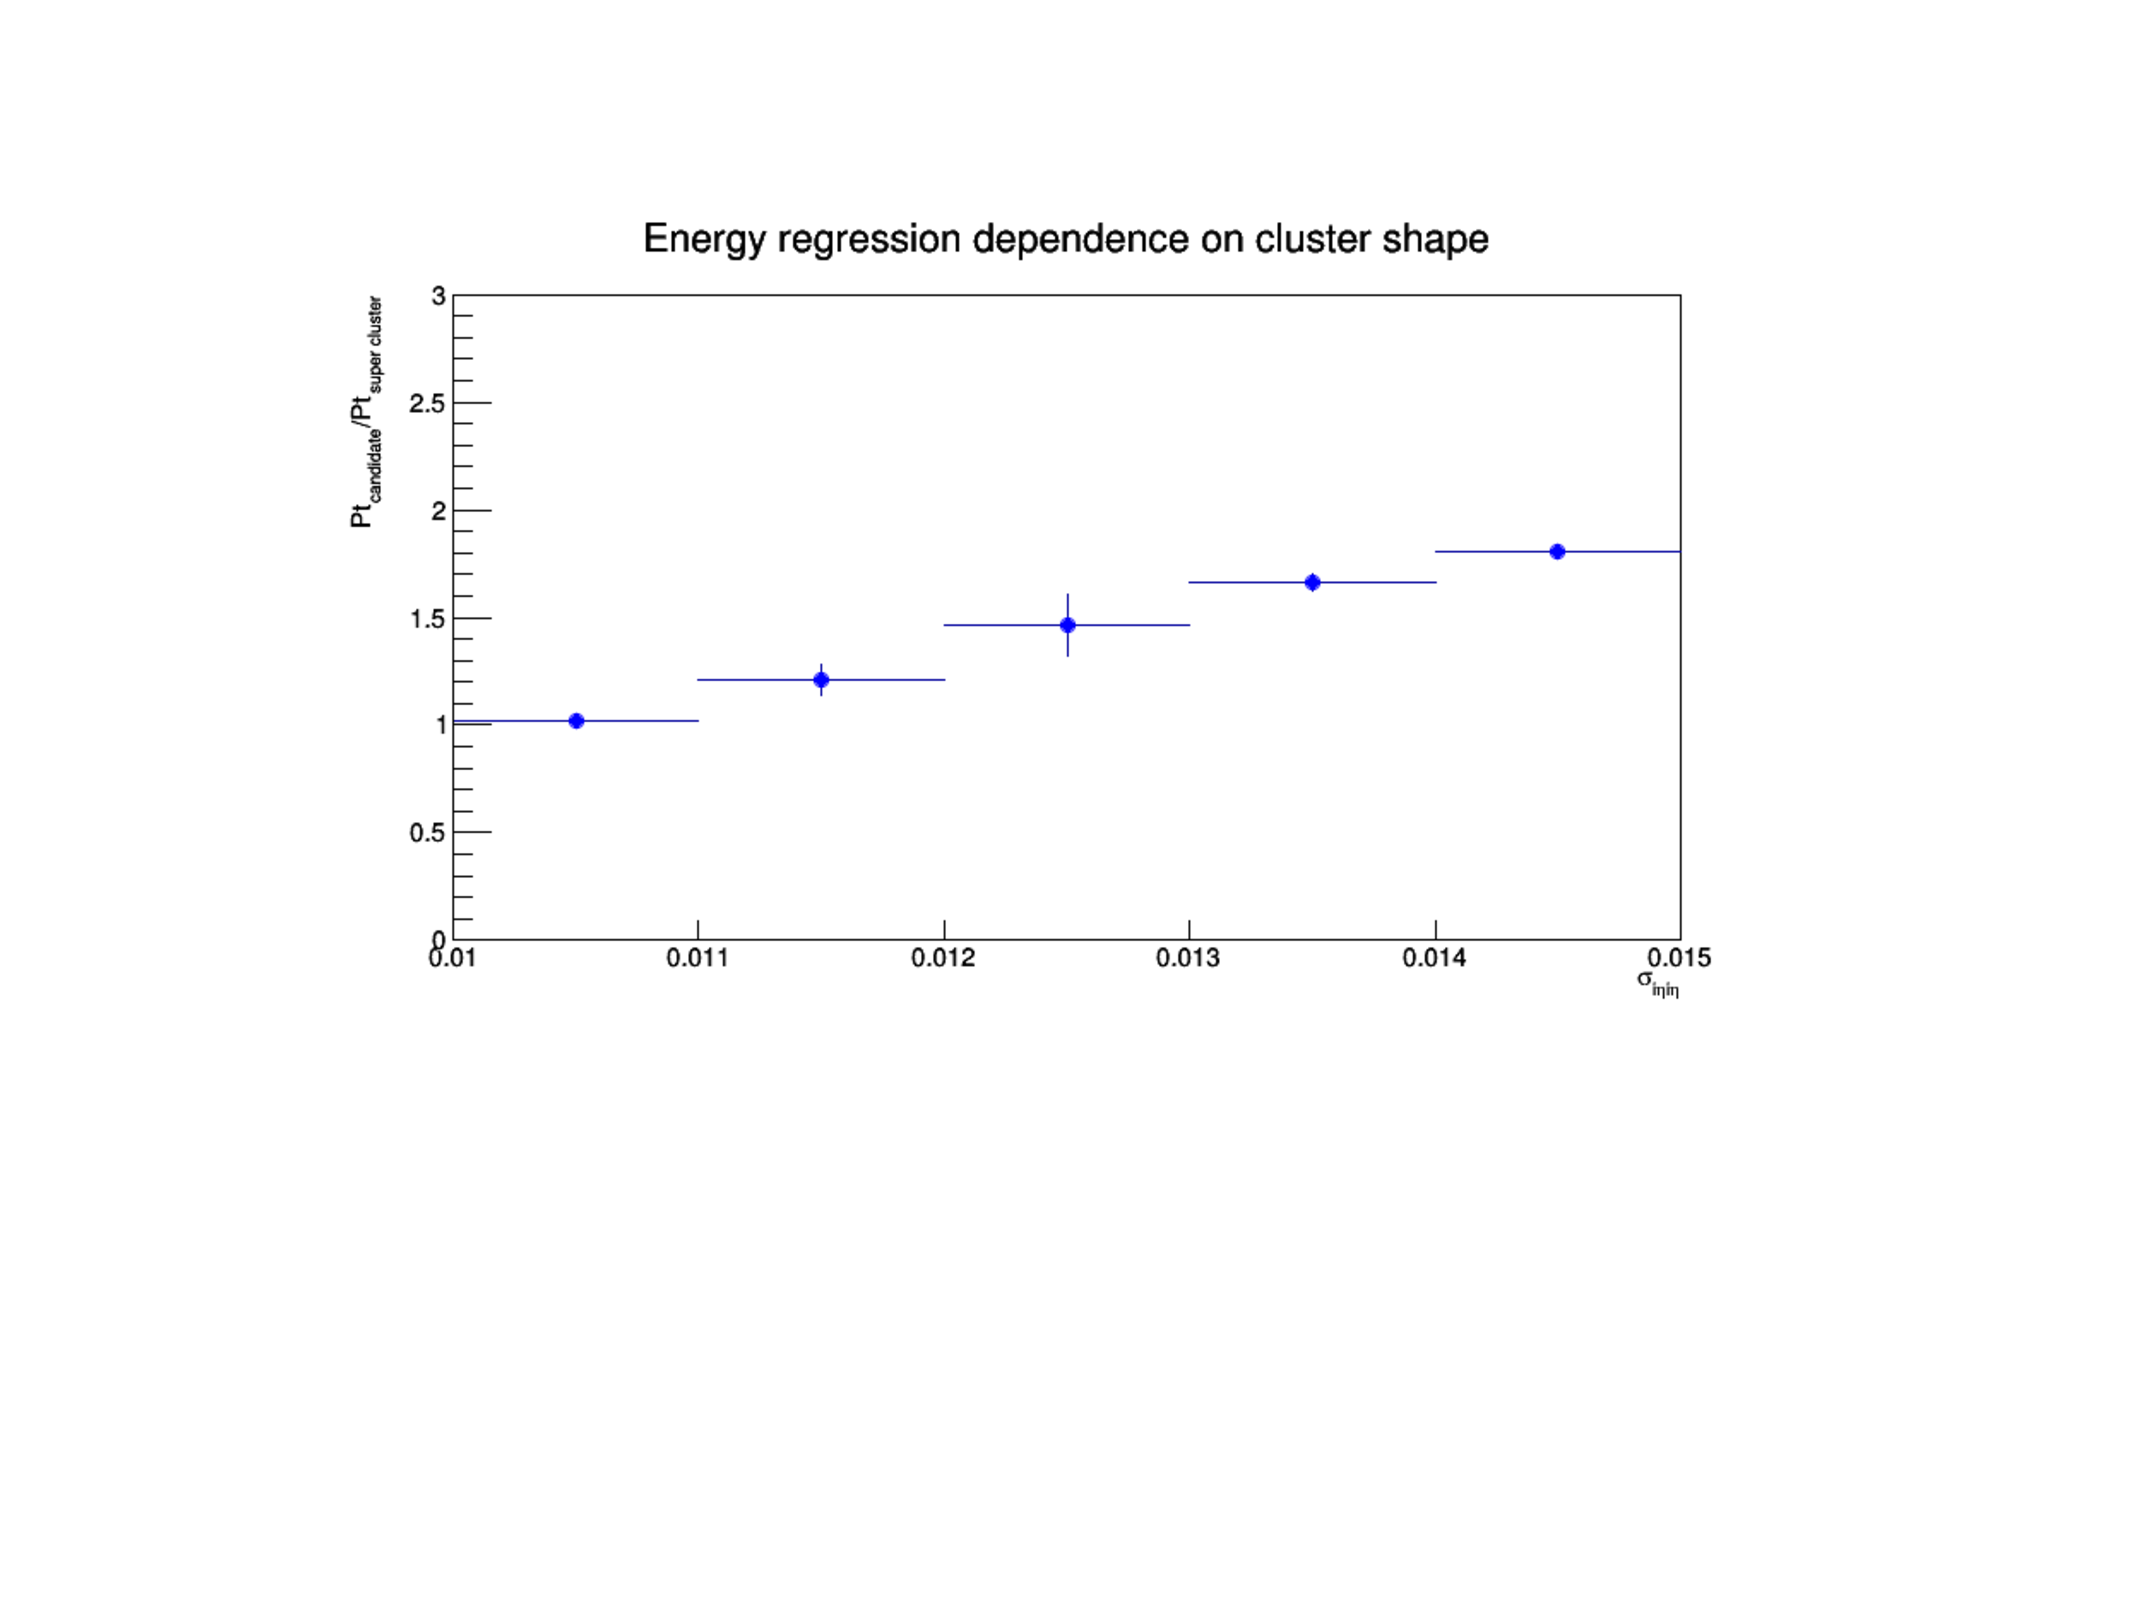
\includegraphics[width=0.6\textwidth]{Reconstruction/Figures/corr_vs_sieie.pdf}
    \caption{
      Magnitude of the energy correction on the photon object in bins of \sieie.
    }
    \label{fig:corr_vs_sieie}
  \end{center}
\end{figure}

As an illustration, an unphysically large correction is causing the transverse momentum of the photon object in the event shown in Fig.~\ref{fig:badcorr_evtdisp} to be nearly twice as large as the transverse momentum imbalance, which is supposed to balance the visible, \ie, photon momentum. 
Photon candidates with wide showers are used to estimate the hadron-to-photon misidentification background, while the photon energy resolution has an insignificant effect. 
Therefore, the unbiased supercluster energy was chosen over the corrected photon energy.

\begin{figure}[htbp]
  \begin{center}
    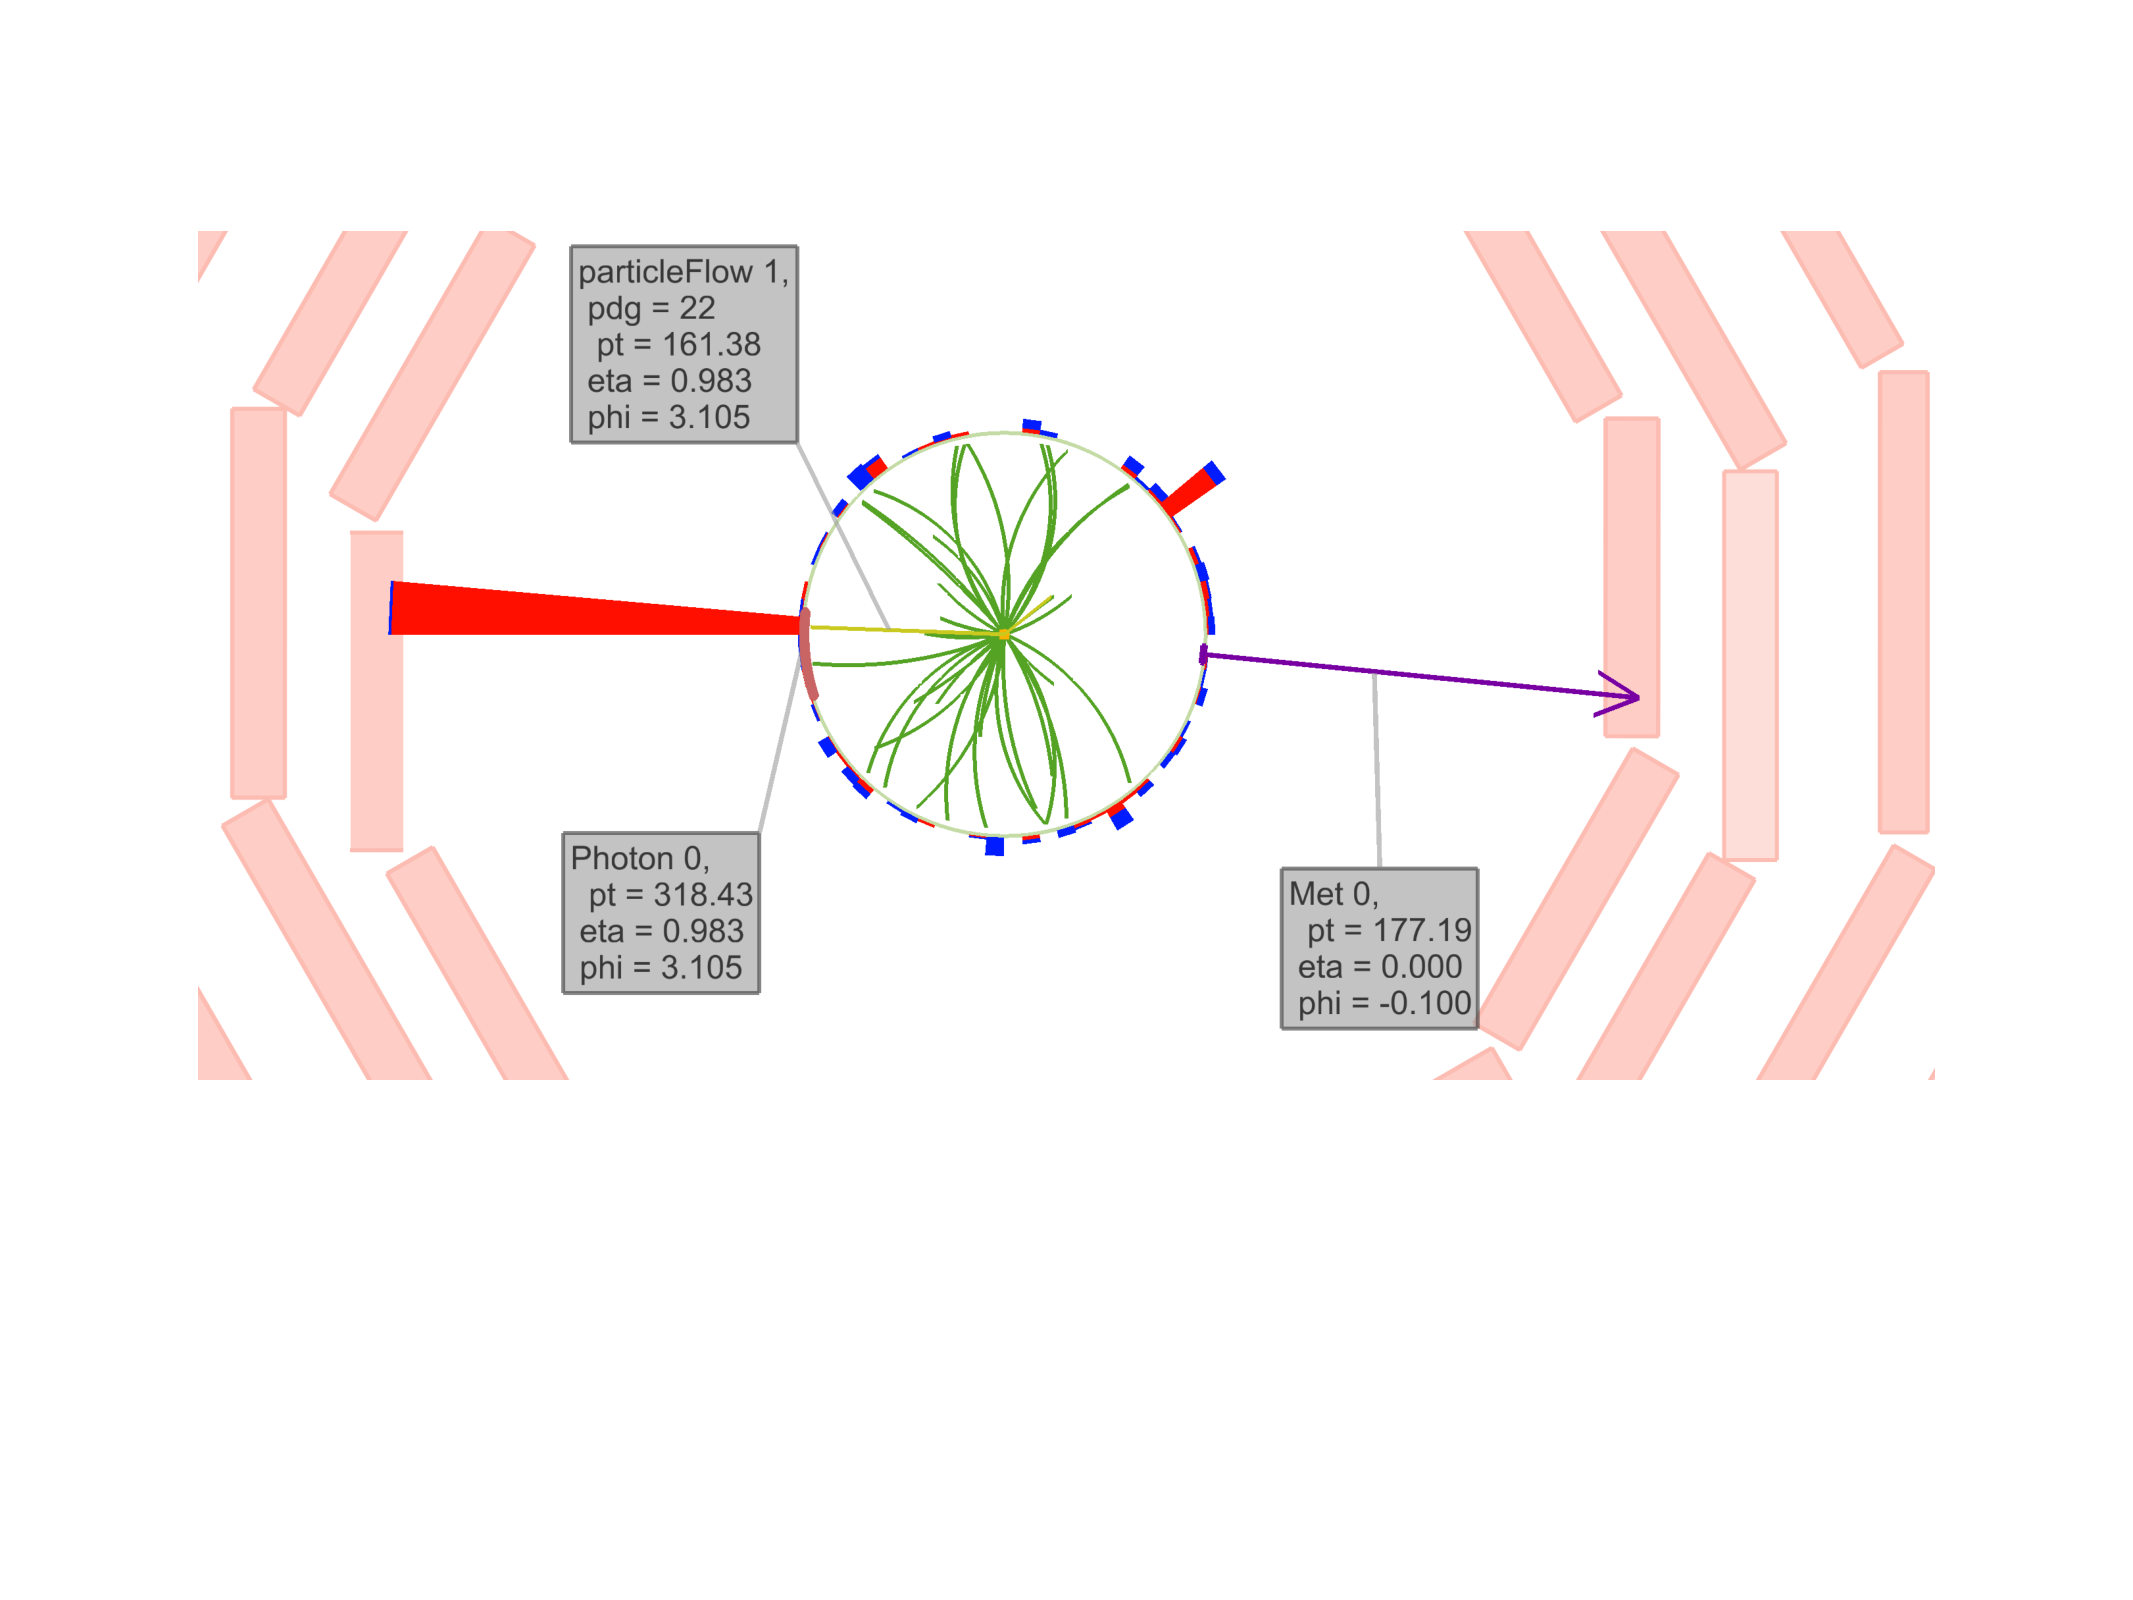
\includegraphics[width=0.6\textwidth]{Reconstruction/Figures/badcorr_evtdisp.pdf}
    \caption{
      An example event where a photon with a wide shower receives a large energy correction.
    }
    \label{fig:badcorr_evtdisp}
  \end{center}
\end{figure}

For the work shown in this thesis, we are only concerned with high-\ET\ photons from the ECAL Barrel that have a supercluster with $\ET > 175\GeV$ and $\abs\eta < 1.4442$. 
To reduce hadron-to-photon misidentification rate, we apply the collection of isolation and shower shape selections in Table~\ref{tab:egid}, which will hereby be referred to as the \egamma\ ID.
To reject electrons from the candidate sample, no electron track seeds in the pixel detector can be associated to the supercluster.
This is known as the pixel seed veto.
To clean the candidate sample from photon objects originating from non-collision sources, we apply the collection of cuts shown in Table~\ref{tab:gsid}, which combined with the pixel seed veto constitutes the \Pgg-specific ID.
The beam halo tagger \emip\ is the total energy deposited in ECAL by a hypothetical beam halo muon that passes through the photon cluster. See Section~\ref{sec:halo} for more detail on beam halo processes. 
The lower bounds on \sieie\ and \sipip\ as well as the requirement on the cluster seed time $\abs\tseed$ are employed to reject spurious photon objects arising from the ``ECAL spikes'' discussed in Section~\ref{sec:spikes}.

\begin{table}[htbp]
  \begin{center}
    \begin{tabular}{l | r}
      Variable & Maximum Value \\
      \hline
      $H/E$ &  0.0260 \\ 
      $\sieie$ &  0.01040 \\ 
      $\rho$-corrected \ICHmax\ & 1.146 \\
      $\rho$-corrected \INH\ & $2.792 + 0.0112 \times \ETg + 0.000028 \times \left(\ETg \right)^2$ \\ 
      $\rho$-corrected \Ig\ & $2.176 + 0.0043 \times \ETg$
    \end{tabular}
    \caption{Selections for the \egamma\ portion of the photon ID. Isolation values and \ETg\ are all in units of \GeV.}
    \label{tab:egid}
  \end{center}
\end{table}

\begin{table}[htbp]
  \begin{center}
    \begin{tabular}{l | l | r}
      Variable & Selection & Description \\
      \hline
      $\emip\ $ & $< 4.9\GeV$ & ECAL energy from a hypothetical beam halo muon \\
      $\sieie\ $ & $> 0.001$ & non-trivial shower width in the $\eta$-direction \\
      $\sipip\ $ & $> 0.001$ & non-trivial shower width in the $\phi$-direction \\
      $\abs\tseed $ & $< 3\ns$ & timing of the cluster seed relative to bunch crossing
    \end{tabular}
    \caption{Additional selections beyond the pixel seed veto for the \Pgg-specific portion of the photon ID.}
    \label{tab:gsid}
  \end{center}
\end{table}

\subsection{Hadrons}
\label{sec:pf_hadrons}

The last candidates reconstructed in a given block are the charged and neutral hadrons from fragmentation and hadronization, as well as the non-isolated muons and photons produced from their respective decays.

Inside the tracker acceptance of $\abs\eta < 2.5$, all trackless HCAL clusters are reconstructed as neutral hadrons while all trackless ECAL clusters are reconstructed as photons.
The preference towards photons is motivated because photons carry 25\% of the jet energy and neutral hadrons do not interact strongly with the ECAL.
Conversely, outside of the tracker acceptance, it is no longer possible to distinguish charged and neutral hadrons, so any ECAL clusters linked to HCAL clusters are assumed to arise from unidentified charged hadrons.
Thus, only unlinked ECAL clusters are reconstructed as photons and linked ECAL and HCAL clusters are reconstructed as neutral hadrons.

Afterwards, the only remaining PF elements are HCAL clusters linked to one or more tracks and ECAL clusters linked to one of these tracks.
A single charged hadron is constructed for each remaining HCAL cluster, with energy equal to the sum of the ECAL and HCAL clusters and momentum equal to the sum of the individual track momenta.

If the energy of the charged hadron exceeds its momentum by an amount larger than the calometric energy resolution, neutral hadrons and photons are added.
For excesses greater than 500\MeV, a photon with energy equal to the excess is created.
If this photon cannont explain the entire excess, e.g. the excess is larger than the ECAL energy by at least 1\GeV, the remainder is indentified as a neutral hadron. 
After photons and neutral hadrons consume the excess calometric energy, charged hadrons are constructed from the linked tracks with their energy and momentum determined by the track momenta under the charged-pion hypothesis. 

If energy and momentum of the charged hadron are compatible, no neutral particles are identified. A charged hadron candidate is created for each track linked to the HCAL cluster, with momenta determined by a $\chi^2$ fit of the tracker and calorimeter measurements.
This combintation ensures a smooth transition between the tracker-dominated low-enrgy regime and the calorimeter-dominated high-energy regime while always improving the final energy resolution. 

If the momentum of the charged hadron exceeds its energy by three standard deviations, new PF muons are made from any non-isolated global muons failing the cleaning described in Section~\ref{sec:pf_muons} with momentum resolution better than 25\%.
If, after masking the tracks from these muons, the track momentum sum still greatly exceeds the calorimeter energy, all remaining tracks with a \pt\ uncertainty greater than 1\GeV are identified, sorted in decreasing order of this uncertainty, and sequentially masked until no such tracks remain or the momentum excess disappears, whichever comes first. 
At this point, the HCAL cluster is reconstructed according to one of the procedures defined in the preceding paragraphs.

When three or more charged particle candidates are linked to a secondary vertex identified as described in Section~\ref{sec:pf_csv}, a single primary charged hadron with energy equal to the sum of their energies replaces them in the reconstructed particle list.
If an incoming track is associated with the vertex, it determines the direction of the primary charged hadron, which is otherwise determined by the vectorial sum of momenta of the secondary particles.
If the momentum of the incoming track is well measured, the energy of undetected secondary particles is estimated and added to the energy of the primary charged particle.

\subsection{Jets}
\label{sec:pf_jets}

As discussed in Section~\ref{sec:collider_pheno}, jets are produced during the fragmentation and hadronization of colored particles produced in the hard scattering.
After all PF candidates have been identified, a sequential recombination algorithm is used in an attempt to cluster these jets.
Given an object $i$ in the event $E$, we define the distance to the beam and the distance to another object $j$ to be
\begin{equation}
  \begin{matrix}[l | r]
    \displaystyle
    d_{iB} = \left(\pt^i\right)^{2q} &
    d_{ij} = \min \left\{\left(\pt^i\right)^{2q}, \left(\pt^j\right)^{2q} \right\} \dfrac{\left(\dR_{ij}\right)^2}{R^2} ,
  \end{matrix}
\end{equation}
respectively, where $q$ and $R$ are tunable parameters and $\dR_{ij}$ is the angular distance between the two particles.
The distance parameter $R$ is an appromixate measure of the cone size \dR\ of the jet, while the power of the energy scale $q$ defines the relationship between the relationship between the momentum and angular factors.
Jets clustered with $q = -1$ are referred to as anti-\kt\ jets, those with $q = 0$ as Cambridge-Aachen jets, and those with $q = 1$ as \kt\ jets.  
Negative values of $q$ force the clustering of circular jets around hard seeds ensuring that the resulting jet boundaries are resilient with respect to soft radiation.
Within CMS, anti-\kt\ jets with $R = 0.4$ are used to cluster the parton shower from single partons.

The implementation in the FastJet library reduces the computational complexity of clustering from $\mathcal{O}(N^2)$ to $\mathcal{O}(N \log N)$ for jets with hundreds or thousands of constituent particles.
First, the two objects $i$ and $j$ with the smallest distance $d_{ij}$ between them are found. 
If $d_{ij}$ is less than both $d_{iB}$ and $d_{jB}$, they are removed from $E$ and a single object $k$ with four-momentum $p_\mu^k = p_\mu^i + p_\mu^j$ which is added in their place. 
Otherwise if $d_{iB} < d_{jB}$, object $i$ is removed from $E$ and added to the set of jet candidates $J$ while object $j$ is kept, and vice versa if $d_{jB} < d_{iB}$.
This procedure continues until all objects are removed from $E$ and $J$ contains all possible jet candidates.

\subsection{Missing Tranverse Energy}
\label{sec:pf_met}

The production of neutrinos and dark matter candidates produces a momentum imbalance in the transverse plane.
The missing transverse momentum \ptvecmiss\ is defined as the negative vectorial sum of all the PF candidates in the event $E$ such that
\begin{equation}
  \ptvecmiss = - \sum_{i\in E} \Big( \hat x \cdot \pt^i \cos \phi + \hat y \cdot \pt^i \sin \phi \Big),
\end{equation}
and its magnitude is the missing transverse energy $\met = \abs\ptvecmiss$.
In a perfectly reconstructed event, non-zero \met\ implies the presence of neutrinos or DM candidates; however, the failure to properly reconstruct energy deposits or the reconstruction of PF candidates with incorrect energy results in events with large amount of fake \met.

One last cleaning of the PF candidates is conducted in an attempt to fix these events.
To remove muons from cosmic rays, muon candidates with trajectories more than 1\cm away from the beam axis are removed if the measured \met\ is consequently reduced by half.
For muons with $\pt > 20\GeV$, the choice of subdetector used to estimate momemtum is reviewed and the smallest available estimate used if it reduces the measured \met\ by half.
Additionally, the assignment of charged hadrons and neutral hadrons is reconsidered to ensure a charged hadron is not reconstructed as a muon and neutral hadron and vice versa.

Fake \met\ can persist in an event even after the final cleaning of PF candidates.
At this point, events are checked against a known set of filters identifying possible sources of fake \met\ not captured by the PF algorithm.
One set of filters is the HCAL and ECAL filters that identify events with calorimeter clusters caused by noise from the shape and timing of the energy distribution.
Another such filter is the beam halo filter that identifies energy deposits from muons produced from interactions between the beam and the machine that travel parallel to the beam. These muons are identified by their localization in $\phi$ and a longitudinal track left in the ECAL endcaps and the CSCs.
Applying these filters removes essentially all remaining events with fake \met\ while rejecting less than 1\% of events with real \met.

\section{Reconstruction Issues}
\label{sec:issues}

This thesis focuses on events with a single high-\pt\ photon and large \met.
There are a lot of reconstruction issues specific to this final state as photons are relatively easy to fake through other processes that result in a large amount of fake \met.
This section describes the three main sources of correlated fake photons and fake \met encountered during this analysis.

\subsection{ECAL gain-switch effect}
\label{sec:gainswitch}

\begin{figure}[htbp]
  \centering
  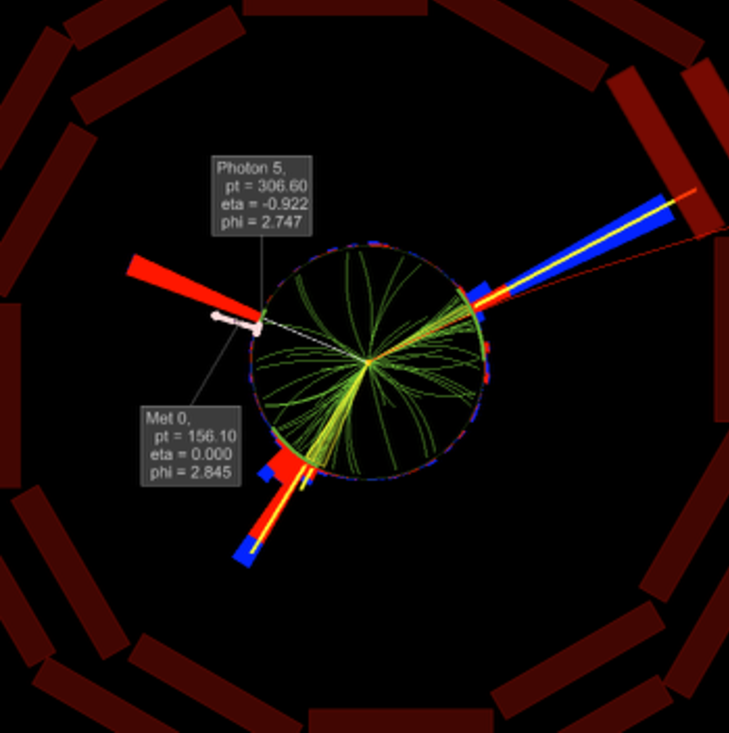
\includegraphics[width=0.48\linewidth]{Reconstruction/Figures/gsfix/evdisp_before.pdf}
  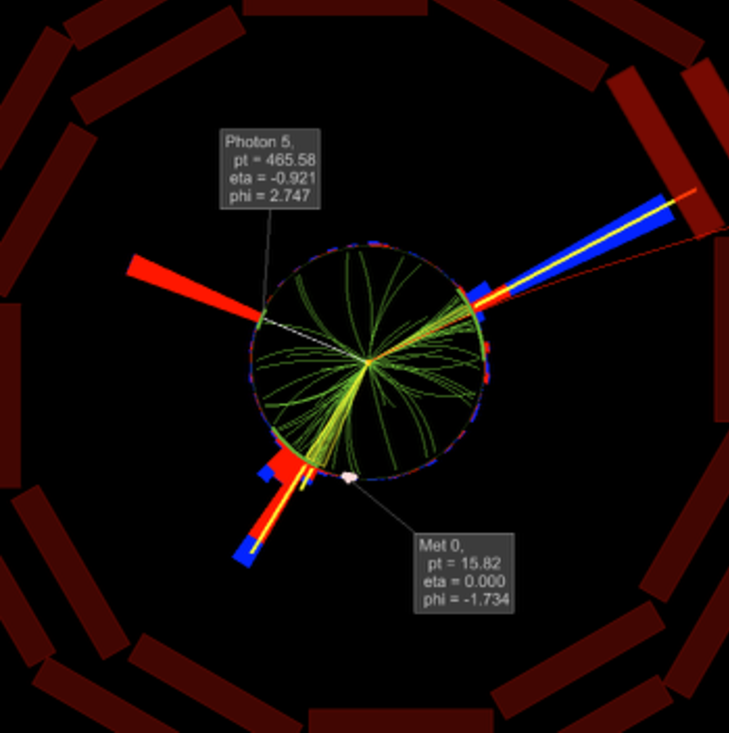
\includegraphics[width=0.48\linewidth]{Reconstruction/Figures/gsfix/evdisp_after.pdf}
  \caption{
    Two event displays comparing the same event, reconstructed without (left) and with (right) the fix for ECAL gain-switch effect.
  }
  \label{fig:eventdisplay_gsfix}
\end{figure}

The ``multi-fit'' algorithm for ECAL hit reconstruction was found to have an unexpected behavior when there is a large energy deposit onto a single ECAL crystal, such that the electronic signal converted at the frontend electronics is sourced partially from channels of the preamplifier with lower gains (6 or 1) than the default (12) channel. 
In the most dramatic cases, pulse misreconstruction would result in underestimation by hundreds of \GeV of photon \pt. 
This effect is mitigated in the reprocessed data set used for this analysis by identifying ECAL clusters whose seed crystal hit had a switch of gains, and performing an alternative pulse reconstruction when possible.

\begin{figure}[htbp]
  \centering
  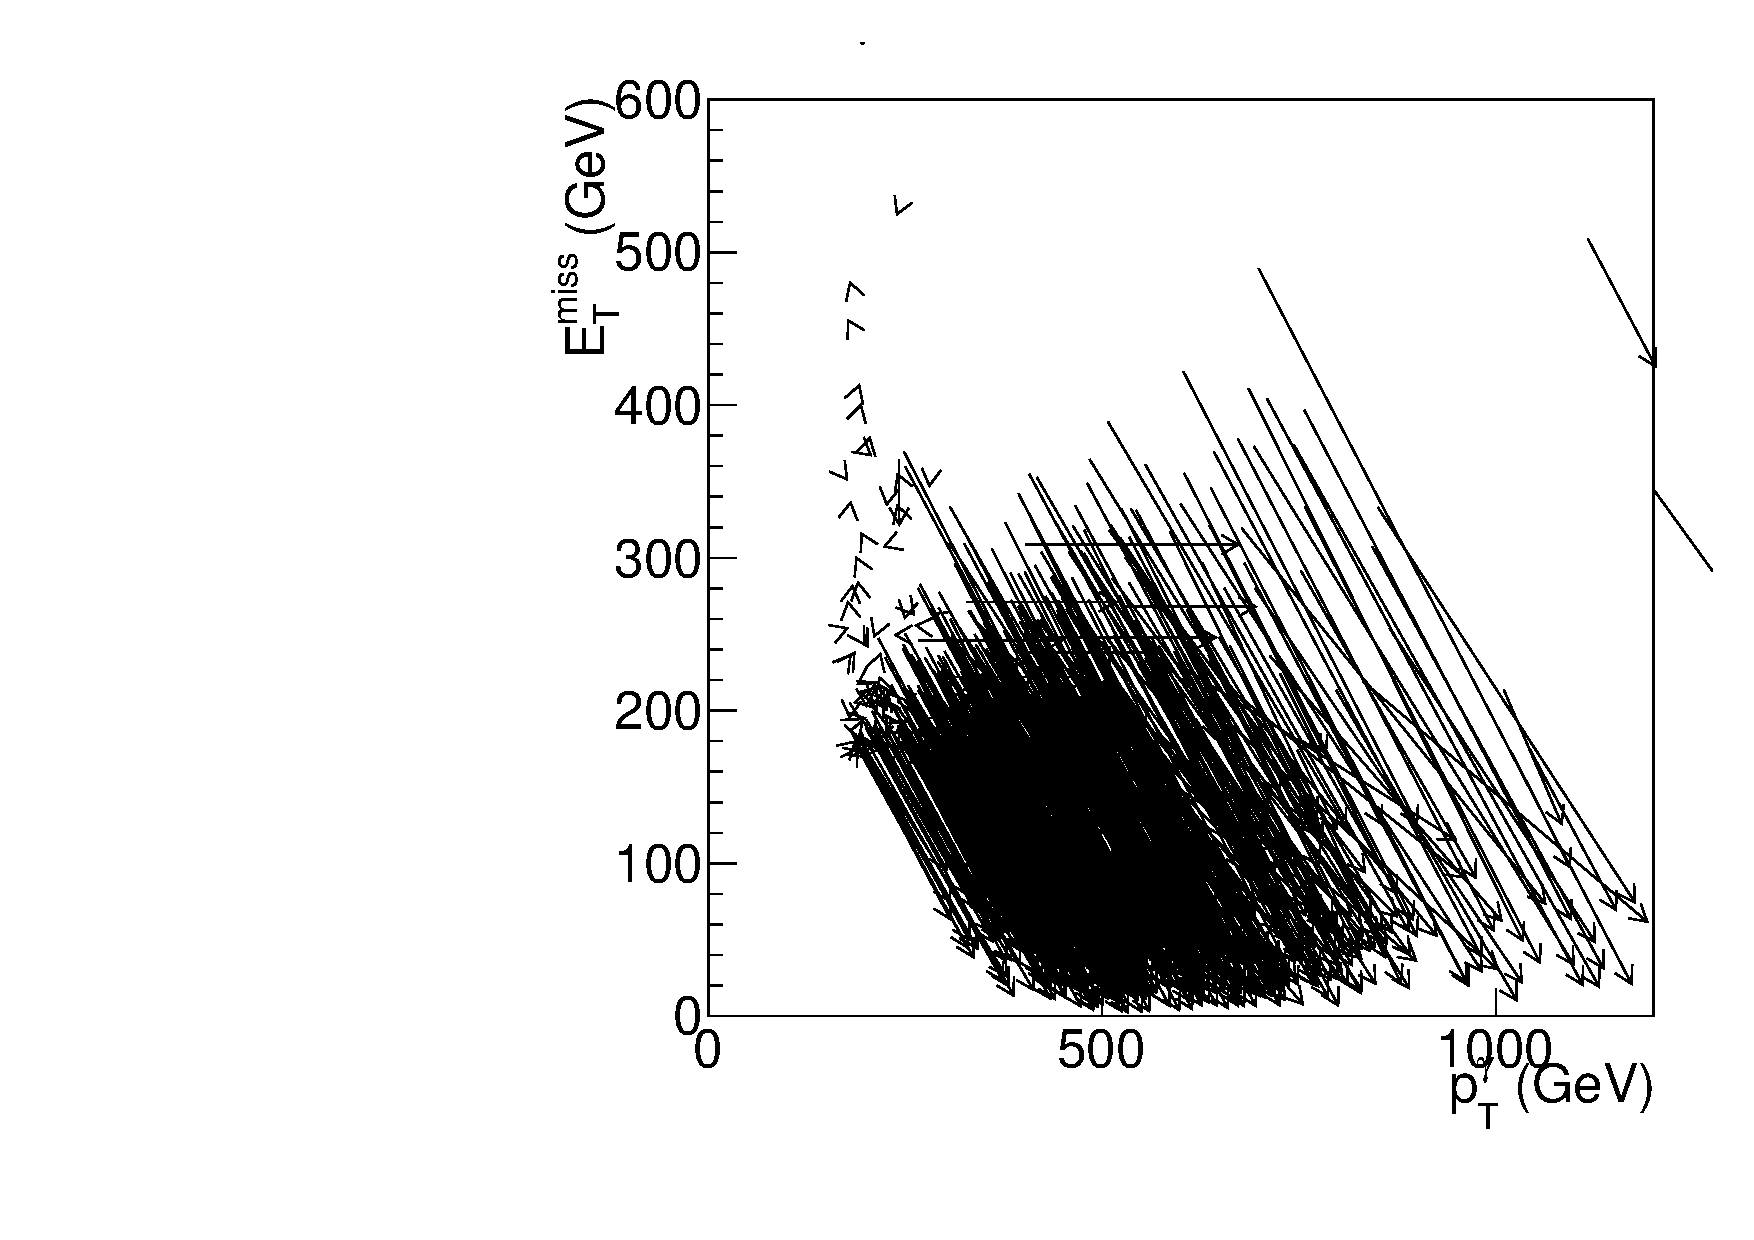
\includegraphics[width=0.6\linewidth]{Reconstruction/Figures/gsfix/movements.pdf}
  \caption{
    The change in reconstructed photon \pt\ and \met\ for events in the bin $\dphigmet < 0.05$ of the distribution in Figure~\ref{fig:dphigmet_beforegsfix}. 
    Each arrow represents a single event, the the tail (head) of the arrow corresponding to (\ETg, \met) coordinates in the datasets without (with) the fix for the gain-switch problem.
  }
  \label{fig:ptshift_gsfix}
\end{figure}

The gain-switch problem affected the analyses documented in this thesis, since large underestimation of the energy of a photon in an otherwise typical \gj\ event would introduce large missing transverse momentum to the event, typical collinear to the affected photon. 
Figures~\ref{fig:eventdisplay_gsfix} and~\ref{fig:ptshift_gsfix} are the visualization of how the new dataset changes the reconstructed photon energy and \met.
